\section{Directory-based Persistence Techniques}\label{section:call signatures dp}
In this section, we will discuss Call Signatures for \autoref{DP0}

In \autoref{DP0}, malware places an executable file (or a link to an executable file) in \path{<User Directory>\AppData\Roaming\Microsoft\Windows\Start Menu\Programs\Startup} to start the executable when the user logs in.

The path of special directories (e.g. the startup directories or a directory for temporary storage) might change between Windows versions. To solve this, the Windows API provides multiple functions that allow applications to resolve the path of special directories. This improves the backward compatibility of applications that use these special directories

To write to the startup directory, malware can either use the path directly or can use a Windows API function to resolve the path of the startup directory.

\subsection{Using the Path of the Startup Directory Directly}
If malware uses the path directly, we are looking for function calls that have the path as a string argument. The Call Signature in \autoref{listing:call signature user startup path} describes such function calls.

\begin{lstlisting}[label={listing:call signature user startup path}, caption={A Call Signature for \autoref{DP0}.}, captionpos=b]
---

signature:
    technique: "DP0"
    description: >
      This Call Signature can be used to
      search for calls that directly use the path of
      the startup directory in a user's directory.
    rules:
        - element: "any argument"
          contains: "AppData\\Roaming\\Microsoft\\Windows\\Start Menu\\Programs\\Startup"
\end{lstlisting}

\subsection{Resolving the Path of the Startup Directory}
From Windows Vista onwards, the API function to resolve the paths of special directories is \texttt{SHGetKnownFolderPath}\footnote{\tiny \url{https://docs.microsoft.com/en-us/windows/win32/api/shlobj_core/nf-shlobj_core-shgetknownfolderpath}}.

This function takes a constant value as its first argument. This constant is a GUID\footnote{\tiny \url{https://docs.microsoft.com/en-us/dotnet/api/system.guid}}, a 16 bytes unique identifier. For example, the identifier that is used to search for the startup directory of the current user is \texttt{B97D20BB-F46A-4C97-BA10-5E3608430854}\footnote{\tiny \url{https://docs.microsoft.com/en-us/windows/win32/shell/knownfolderid}}.

In a binary, a GUID is represented directly by the 16 bytes. \autoref{fig:guid in assembly} shows how the disassembler of IDA Pro interprets the bytes in a GUID.

\begin{figure}[ht]
  \centering
  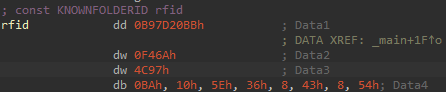
\includegraphics[width=0.7\textwidth]{resources/images/guid_in_assembly.png}
  \caption{A GUID in a binary disassembled by IDA Pro.}
  \label{fig:guid in assembly}
\end{figure}

To detect calls to \texttt{SHGetKnownFolderPath} that resolve the path used in \autoref{DP0}, we need to write a rule that constrains the specific bytes of the GUID in the first argument, like in \autoref{listing:call signature SHGetKnownFolderPath}.

\begin{lstlisting}[label={listing:call signature SHGetKnownFolderPath}, caption={A Call Signature that matches a call to \texttt{SHGetKnownFolderPath}.}, captionpos=b]
---

signature:
    technique: "DP0"
    description: >
      This Call Signature can be used to
      search for calls to SHGetKnownFolderPath.
    rules:
        - element: "function name"
          equals: "SHGetKnownFolderPath"

        - element: "number of arguments"
          equals: 4

        - element: "argument"
          argument_index: 0
          equals: "BB 20 7D B9 6A F4 97 4C BA 10 5E 36 08 43 08 54"
          type: "bytes"
\end{lstlisting}

\subsubsection{Deprecated API Functions}

Before Windows Vista, there were multiple (now deprecated, but still available) functions available to resolve the paths of directories.

All these functions take a constant that represents the startup directory as an argument. This constant is called \texttt{CSIDL\_STARTUP}\footnote{\tiny \url{https://docs.microsoft.com/en-us/windows/win32/shell/csidl}} and its value is 7.

\pagebreak

We write Call Signatures for all of these functions:
\begin{itemize}
    \item \texttt{SHGetFolderPath}\footnote{\tiny \url{https://docs.microsoft.com/en-us/windows/win32/api/shlobj_core/nf-shlobj_core-shgetfolderpathw}}
\begin{lstlisting}[caption={A Call Signature that matches a call to \texttt{SHGetFolderPath}.}, captionpos=b]
---

signature:
    technique: "DP0"
    description: >
      This Call Signature can be used to
      search for calls to SHGetFolderPath.
    rules:
        - element: "function name"
          contains: "SHGetFolderPath"

        - element: "number of arguments"
          equals: 5

        - element: "argument"
          argument_index: 1
          equals: 0x07
\end{lstlisting}


    \item \texttt{SHGetFolderLocation}\footnote{\tiny \url{https://docs.microsoft.com/en-us/windows/win32/api/shlobj_core/nf-shlobj_core-shgetfolderlocation}}
\begin{lstlisting}[caption={A Call Signature that matches a call to \texttt{SHGetFolderLocation}.}, captionpos=b]
---

signature:
    technique: "DP0"
    description: >
      This Call Signature can be used to
      search for calls to SHGetFolderLocation.
    rules:
        - element: "function name"
          contains: "SHGetFolderLocation"

        - element: "number of arguments"
          equals: 5

        - element: "argument"
          argument_index: 1
          equals: 0x07
\end{lstlisting}

\pagebreak

    \item \texttt{SHGetSpecialFolderPath}\footnote{\tiny \url{https://docs.microsoft.com/en-us/windows/win32/api/shlobj_core/nf-shlobj_core-shgetspecialfolderpathw}}:
\begin{lstlisting}[caption={A Call Signature that matches a call to \texttt{SHGetSpecialFolderPath}.}, captionpos=b]
---

signature:
    technique: "DP0"
    description: >
      This Call Signature can be used to
      search for calls to SHGetSpecialFolderPath.
    rules:
        - element: "function name"
          contains: "SHGetSpecialFolderPath"

        - element: "number of arguments"
          equals: 4

        - element: "argument"
          argument_index: 2
          equals: 0x07
\end{lstlisting}

    \item \texttt{SHGetSpecialFolderLocation}\footnote{\tiny \url{https://docs.microsoft.com/en-us/windows/win32/api/shlobj_core/nf-shlobj_core-shgetspecialfolderlocation}}:
\begin{lstlisting}[caption={A Call Signature that matches a call to \texttt{SHGetSpecialFolderLocation}.}, captionpos=b]
---

signature:
    technique: "DP0"
    description: >
      This Call Signature can be used to
      search for calls to SHGetSpecialFolderLocation.
    rules:
        - element: "function name"
          contains: "SHGetSpecialFolderLocation"

        - element: "number of arguments"
          equals: 3

        - element: "argument"
          argument_index: 1
          equals: 0x07
\end{lstlisting}
\end{itemize}
